\documentclass[9pt,letterpaper,onecolumn]{rho-class/rho}
\usepackage[spanish,es-nodecimaldot,es-noindentfirst]{babel}
\setlength{\parindent}{0pt}  % Elimina la sangría
\usepackage[utf8]{inputenc}
\usepackage[T1]{fontenc}
\setbool{rho-abstract}{true} % Set false to hide the abstract
\setbool{corres-info}{true} % Set false to hide the corresponding author section
\addbibresource{rho.bib}

%----------------------------------------------------------
% TITLE
%----------------------------------------------------------

%\journalname{Example Template}
\title{Simulador de Gestión de memoria y planificación de procesos: forKing}

%----------------------------------------------------------
% AUTHORS AND AFFILIATIONS
%----------------------------------------------------------

\author[$\dagger$]{Milton Hernandez}
\author[$\dagger$]{Iván Mansilla}
\author[$\dagger$]{Ayrton Morrison}

%----------------------------------------------------------

%\affil[1]{Affiliation of author one}
%\affil[2]{Affiliation of author two}
%\affil[3]{Affiliation of author three}
\affil[$\dagger$]{Universidad de Magallanes}

%----------------------------------------------------------
% DATES
%----------------------------------------------------------

\dates{Este informe fue compilado el \today}

%----------------------------------------------------------
% FOOTER INFORMATION
%----------------------------------------------------------

%\leadauthor{Author last name et al.}
%\footinfo{Creative Commons CC BY 4.0}
\smalltitle{Estructuras de datos}
%\institution{College name}
\theday{\today} %\today

%----------------------------------------------------------
% ARTICLE INFORMATION
%----------------------------------------------------------

%\corres{Provide the corresponding author information and publisher here.}
%\email{example@organization.com.}
%\doi{\url{https://www.doi.org/exampledoi/XXXXXXXXXX}}

%\received{March 20, 2024}
%\revised{April 16, 2024}
%\accepted{April 20, 2024}
%\published{May 21, 2024}

%\license{Rho LaTeX Class \ccLogo\ This document is licensed under Creative Commons CC BY 4.0.}

%----------------------------------------------------------
% ABSTRACT
%----------------------------------------------------------

\begin{abstract}
    A la hora de trabajar con sistemas operativos es fundamental conocer las Estructuras de Datos que se encuentran involucradas en la gestión de procesos así como los diferentes algoritmos de manejo de estos; materias las cuales facilitan el trabajo del sistema operativo sobre los procesos que los conforman. Por esta razón en el presente informe se describe una simulación simple realizada sobre el lenguaje C de un gestor de memoria y un manejador de procesos con estructuras de datos tales como: Listas enlazadas simples, Colas y Árboles Binarios.
\end{abstract}

%----------------------------------------------------------

\keywords{Estructuras de datos, LES, Buddy System, Colas, forKing}

%----------------------------------------------------------
\begin{document}
    \maketitle
    \thispagestyle{firststyle}
    \tableofcontents
    %\linenumbers
    %----------------------------------------------------------


    \newpage
    \section{Introduction}

\rhostart{F}orking es un simulador de gestión de memoria y planificación de procesos, este hace uso de diversas estructuras de datos, como lo son; Listas en enlazadas simples, colas, arboles, etc. El simulador se encarga de emular la ejecución de procesos en un sistema operativo, pasando por una asignación de memoria, para luego ser procesado con criterios específicos para maximizar la eficiencia del sistema.

Para llevar a buen término el desarrollo de esta aplicación hubo que decidir cuales serían las características que harían de este proyecto uno de interés. Algunas a destacar son:
\begin{enumerate}
    \item \textbf{Cantidad de procesos}: Es importante permitir al usuario especificar el numero de tareas que se encuentran en el sistema, logrando procesar cantidades pequeñas pero también generar simulaciones con cantidades mayores.
    \item \textbf{Tiempo de llegada y tiempo de ejecución}: Es fundamental darle libertad al usuario para especificar el tiempo de llegada de cada proceso, así como el tiempo de ejecución de cada tarea, para hacer simulaciones fieles al comportamiento real.
    \item \textbf{Memoria requerida por cada proceso}: Por supuesto las tareas no ocuparán todas la misma cantidad de memoria RAM por lo que manejar memorias diversas será importante para el buen desarrollo del proyecto.
    \item \textbf{Fragmentación de memoria}: Controlar la fragmentación de memoria puede ser clave para la eficiencia de un sistema operativo, por lo que fue una de las prioridades a la hora de desarrollar esta aplicación.
\end{enumerate}

La elección de los algoritmos de gestión y planificación de procesos fue un punto clave en el desarrollo del proyecto, ya que estos conforman las bases del simulador y son los encargados de hacer que el sistema sea eficiente y funcional. Los algoritmos de gestión de memoria y planificación de tareas elegidos fueron:
\begin{enumerate}
    \item \textbf{BuddySystem}: Algoritmo de gestión de memoria que divide la memoria en bloques de tamaño potencia de 2, permitiendo una asignación de memoria eficiente.
    \item \textbf{RoundRobin}: Algoritmo de planificación de procesos que asigna un tiempo de ejecución a cada proceso, permitiendo que todos los procesos tengan la misma prioridad.
    \item \textbf{ShortestJobFirst}: Algoritmo de planificación de procesos que trabaja proceso que requieren de un \textit{burstime} menor, permitiendo que los procesos mas cortos tengan prioridad.
\end{enumerate}
Mas adelante se profundizará más en el funcionamiento e implementación de cada uno de estos, asi como también en las estructuras de datos utilizadas.

\section{Objetivos}
El objetivo principal de este proyecto es: Construir una simulación de sistema de gestión de memoria y planificación de procesos, mediante el uso de las estructuras de datos vistas en clase.

\subsection{Objetivos secundarios}
\begin{enumerate}
    \item \textbf{Uso de estructuras de datos}: Construir un software funcional, eficiente y bien estructurado, mediante el uso de estructuras de datos, como listas enlazadas, colas, arboles, etc.
    \item \textbf{Eficiencia}: Generar breves tiempos de procesamiento haciendo un uso eficiente de recursos y una elección adecuada de algoritmos.
    \item \textbf{Trabajo en grupo}: Reforzar el trabajo en equipo, asignando roles y tareas a cada miembro del equipo.
    \item \textbf{Planificación de tareas}: Dividir el proyecto en tareas atómicas que permitan su realización de manera más efectiva, asignando tiempos y recursos a cada una de estas.
\end{enumerate}


    \newpage
    \section{Planteamiento del desarrollo del proyecto}
\rhostart{P}ara llevar a cabo el proyecto forKing fue necesario comprender cuál era el objetivo final al que se deseaba llegar razón por la cuál se ha decidido dividir el trabajo en dos fases: Gestión de memoria y planificación de procesos.


\subsection{Gestión de memoria}
En este punto fue necesario plantearse la manera en que se simularía la memoria dentro de forKing; ¿Se usaría memoria real a través de \texttt{Malloc()}? o tal vez ¿Podemos simular la memoria con un \textit{arreglo estático} donde asignar a cada uno de sus elementos una ``cantidad de memoria`` determinada?

Luego de investigar la gestión de memoria en diversos sistemas operativos se optó por hacer una implementación sencilla del sistema usado por \texttt{Linux}, el \textbf{BuddySystem} el cuál consiste en lo siguiente:
\begin{itemize}
    \item Se asume la memoria como un gran bloque de espacio disponible, supondremos un ejemplo con $2048$ bytes de memoria.
    \item Esta memoria construida tiene la capacidad de dividirse de manera \textit{binaria} recursivamente, lo que quiere decir, en el caso del ejemplo, que se pueden tener:
    \begin{itemize}
        \item Hasta $1$ bloque de $2048$ bytes
        \item Hasta $2$ bloques de $1024$ bytes
        \item Hasta $4$ bloques de $512$ bytes
        \item Hasta $8$ bloques de $256$ bytes
        \item Hasta $16$ bloques de $128$ bytes
        \item Hasta $32$ bloques de $64$ bytes
        \item Hasta $64$ bloques de $32$ bytes
        \item Etc$\dots$
    \end{itemize}
    \item Cuando un proceso requiere entrar en el BuddySystem se busca el bloque de memoria más cercano a la cantidad de memoria requerida (por encima) y asigna la memoria a dicho proceso, por ejemplo, si llegara un proceso que requiere de $500$ bytes de memoria, se asignaría un bloque de memoria de $512$ bytes, ya que este es el tamaño de bloque más cercano.
    \item Es aquí donde la división entra en juego. Si no existe un bloque de $512$ bytes de memoria, pero sí uno de $1024$ bytes, entonces este se dividirá en dos bloques de $512$ bytes, uno de los cuales será ocupado por el proceso, y el otro quedará libre para ser usado o fragmentado de ser necesario.
    \item Cuando un bloque se divide en dos más pequeños diremos que estos son \textit{Buddys} el uno del otro.
    \item En caso de que un proceso termine de usar un bloque de la memoria este queda libre. En este momento se evalúa si su \textit{Buddy} también está libre y, de ser así ambos se juntan generando un bloque más grande.
\end{itemize}

\begin{figure}[!ht]
    \centering
    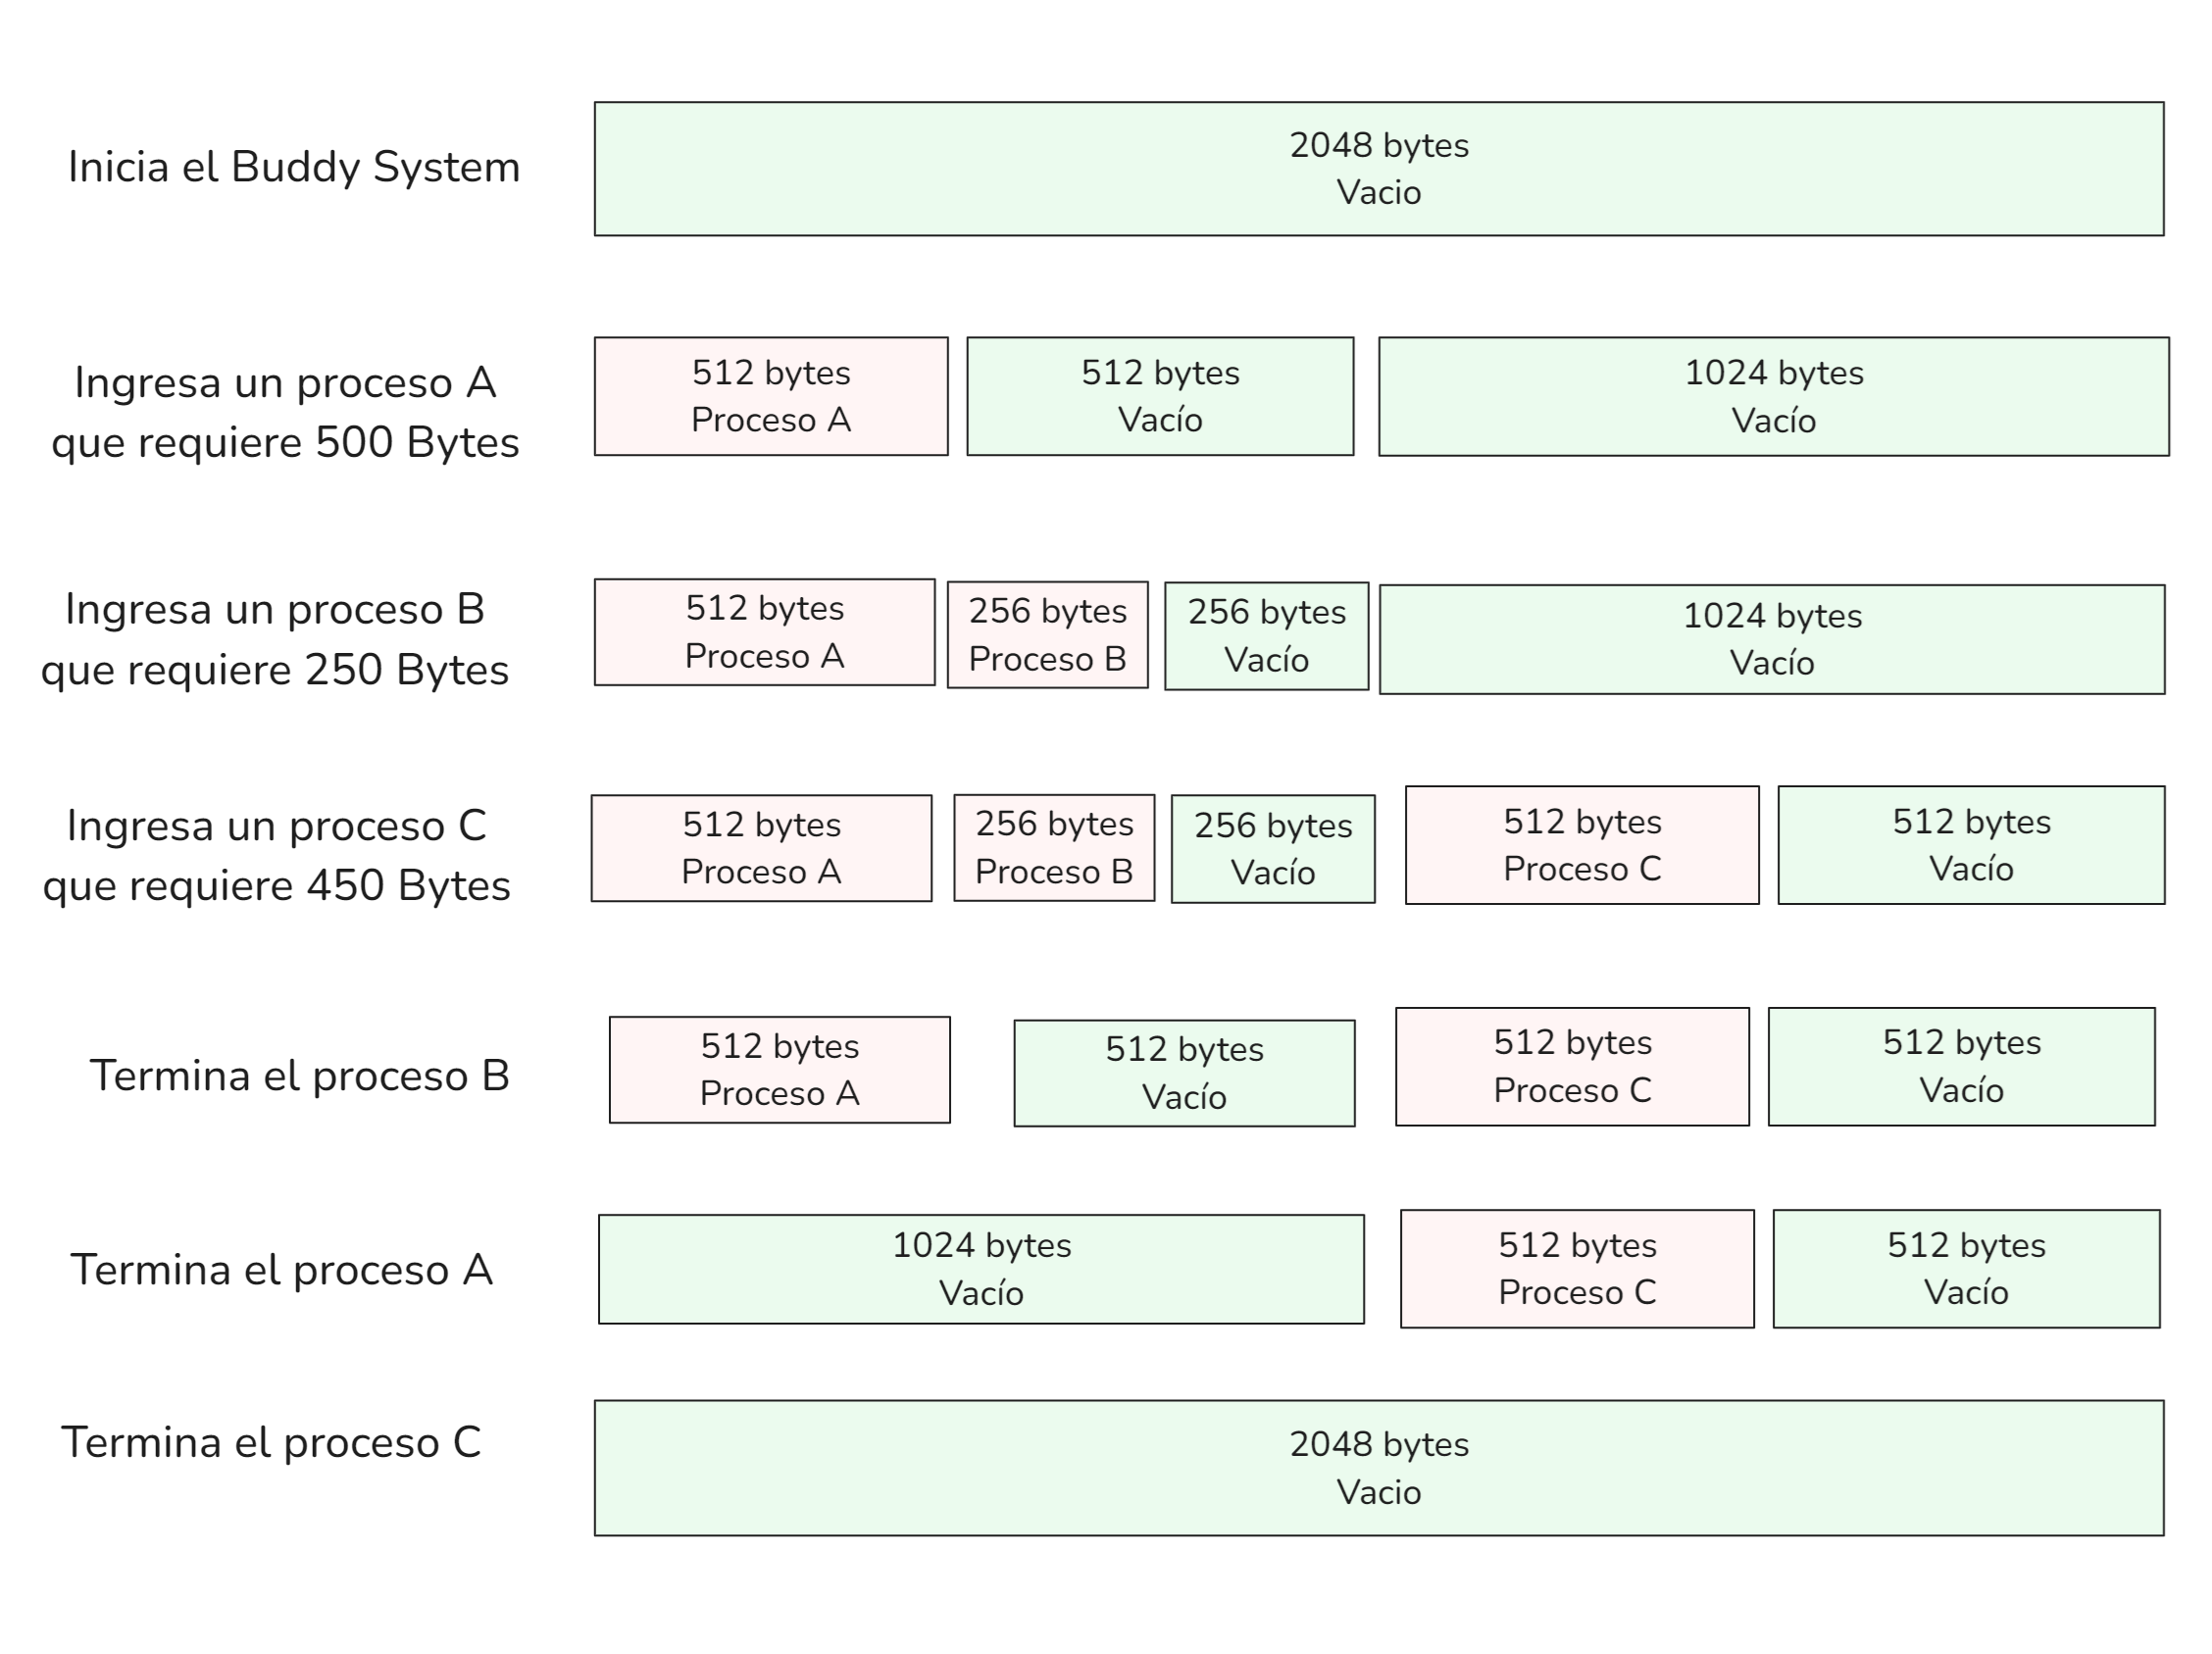
\includegraphics[width=0.8\textwidth]{src/figures/BuddyExample.png}
    \caption{Ejemplo de funcionamiento del buddySystem}\label{fig:buddyexample}
\end{figure}

\begin{note}
    Cada bloque dentro del \textit{BuddySystem} cuanta con una característica conocida como \textbf{Orden del bloque}, donde:

    Un bloque que no se puede dividir tendrá orden $0$ Y el orden irá ascendiendo hasta llegar al bloque más grande posible que tendrá el orden más alto posible.
\end{note}

¿Cuales son las ventajas de la utilización de un \textit{BuddySystem}? Principalmente que este sistema permite manejar de manera muy eficiente el fenómeno de la \textbf{Fragmentación de memoria} que ocurre que cuando procesos que requieren poca memoria terminan de ser procesados dejando partes muy pequeñas de la memoria vacías, lo que genera que, cuando un proceso que requiera de mucha memoria desee ser procesado, no encuentre un lugar lo suficientemente grande para ubicarse dentro de la memoria.

En la figura\ref{fig:buddyexample} se puede ver el comportamiento de un \textit{BuddySystem} de este tipo de manera gráfica.

\subsection{Manejo de procesos}
Una vez que ya tenemos una lista de procesos listos para su ejecución necesitamos de una manera eficiente para procesarlos. Una posible opción sería usar el algoritmo \texttt{FCFS} que consiste en atender a los procesos en el orden de llegada, sin embargo no es del todo eficiente, puesto que si llega un proceso que tarda $100s$ en ser ejecutado y detrás viene uno que tarda $10s$ este segundo deberá esperar demasiado tiempo para su ejecución.

Por esta razón surge el algoritmo \texttt{Shortest Job First} que consiste en atender a los procesos en el orden de su tiempo de ejecución (\texttt{burstTime}), sin embargo esto puede provocar que los procesos con mucho tiempo de ejecución no sean ejecutados nunca.

Para solucionar este último inconveniente aparece el algoritmo \texttt{Round Robin} donde todos los procesos sean parcialmente atendidos, dando como mínimo a cada uno $n$ ráfagas de CPU (\texttt{ticks}), donde $n$ es conocido como \texttt{quantum}. Así no existen procesos con tiempos de ejecución muy altos que no sean ejecutados.

En el presente proyecto se optó por el uso combinado de los algoritmos \texttt{Shortest Job First} y \texttt{Round Robin} en un modelo conocido como \textbf{algoritmo de colas multinivel} donde para un mismo Sistema Operativo se usan diversas colas que permiten un procesamiento eficiente de los recursos. El funcionamiento que se decidió dar al programa es el siguiente:

\begin{itemize}
    \item Un proceso cuyo \texttt{burstTime} es menor al \texttt{quantum} designado entra directamente a la cola \texttt{sjfQueue}.
    \item Un proceso cuyo \texttt{burstTime} es mayor o igual al \texttt{quantum} va a una cola que recibe el nombre de \texttt{rrQueue}.
    \item Si el \texttt{quantum} termina y el proceso sobre el que se trabajó tiene un tiempo restante menor al \texttt{quantum} va directamente a la \texttt{sjfQueue}.
    \item Por último la \texttt{sjfQueue} tiene más prioridad que la \texttt{rrQueue}, de forma que los procesos cortos se atienden primero y los largos se atienden mediante el \texttt{Round Robin}.
\end{itemize}

\subsection{Planificación general del proyecto}
Conociendo ya los conceptos usados en el proyecto resta solamente comentar cómo será la ejecución del programa, sin embargo antes se aclararán algunos conceptos adicionales propios del proyecto.
\begin{itemize}
    \item \textbf{ArrivalQueue}: Es una cola donde se almacenan los procesos que llegan a la simulación (Se asume que un proceso llega a la simulación si su \texttt{arrivalTime} coincide con la cantidad de \texttt{ticks} que han transcurrido desde que se inició el programa).
    \item \textbf{WaitingQueue}: Es una cola donde se almacenan los procesos que están esperando a ser procesados (Un proceso entra a esta cola si no existe memoria en el \texttt{BuddySystem} para este).
    \item \textbf{RRQueue}: Es una cola donde se almacenan los procesos que deben ser procesados por \texttt{Round Robin}.
    \item \textbf{SJFQueue}: Es una cola donde se almacenan los procesos que deben ser procesados por \texttt{Shortest Job First}.
    \item \textbf{BuddySystem}: Estructura de datos que representa el \textit{sistema} de buddies descrito anteriormente.
\end{itemize}

Con todas estas herramientas se describe el funcionamiento de \textit{forKing} en la figura \ref{fig:flowchart} donde se omiten comprobaciones varias de las colas para simplificar el diagrama.

\begin{figure}[!ht]
    \centering
    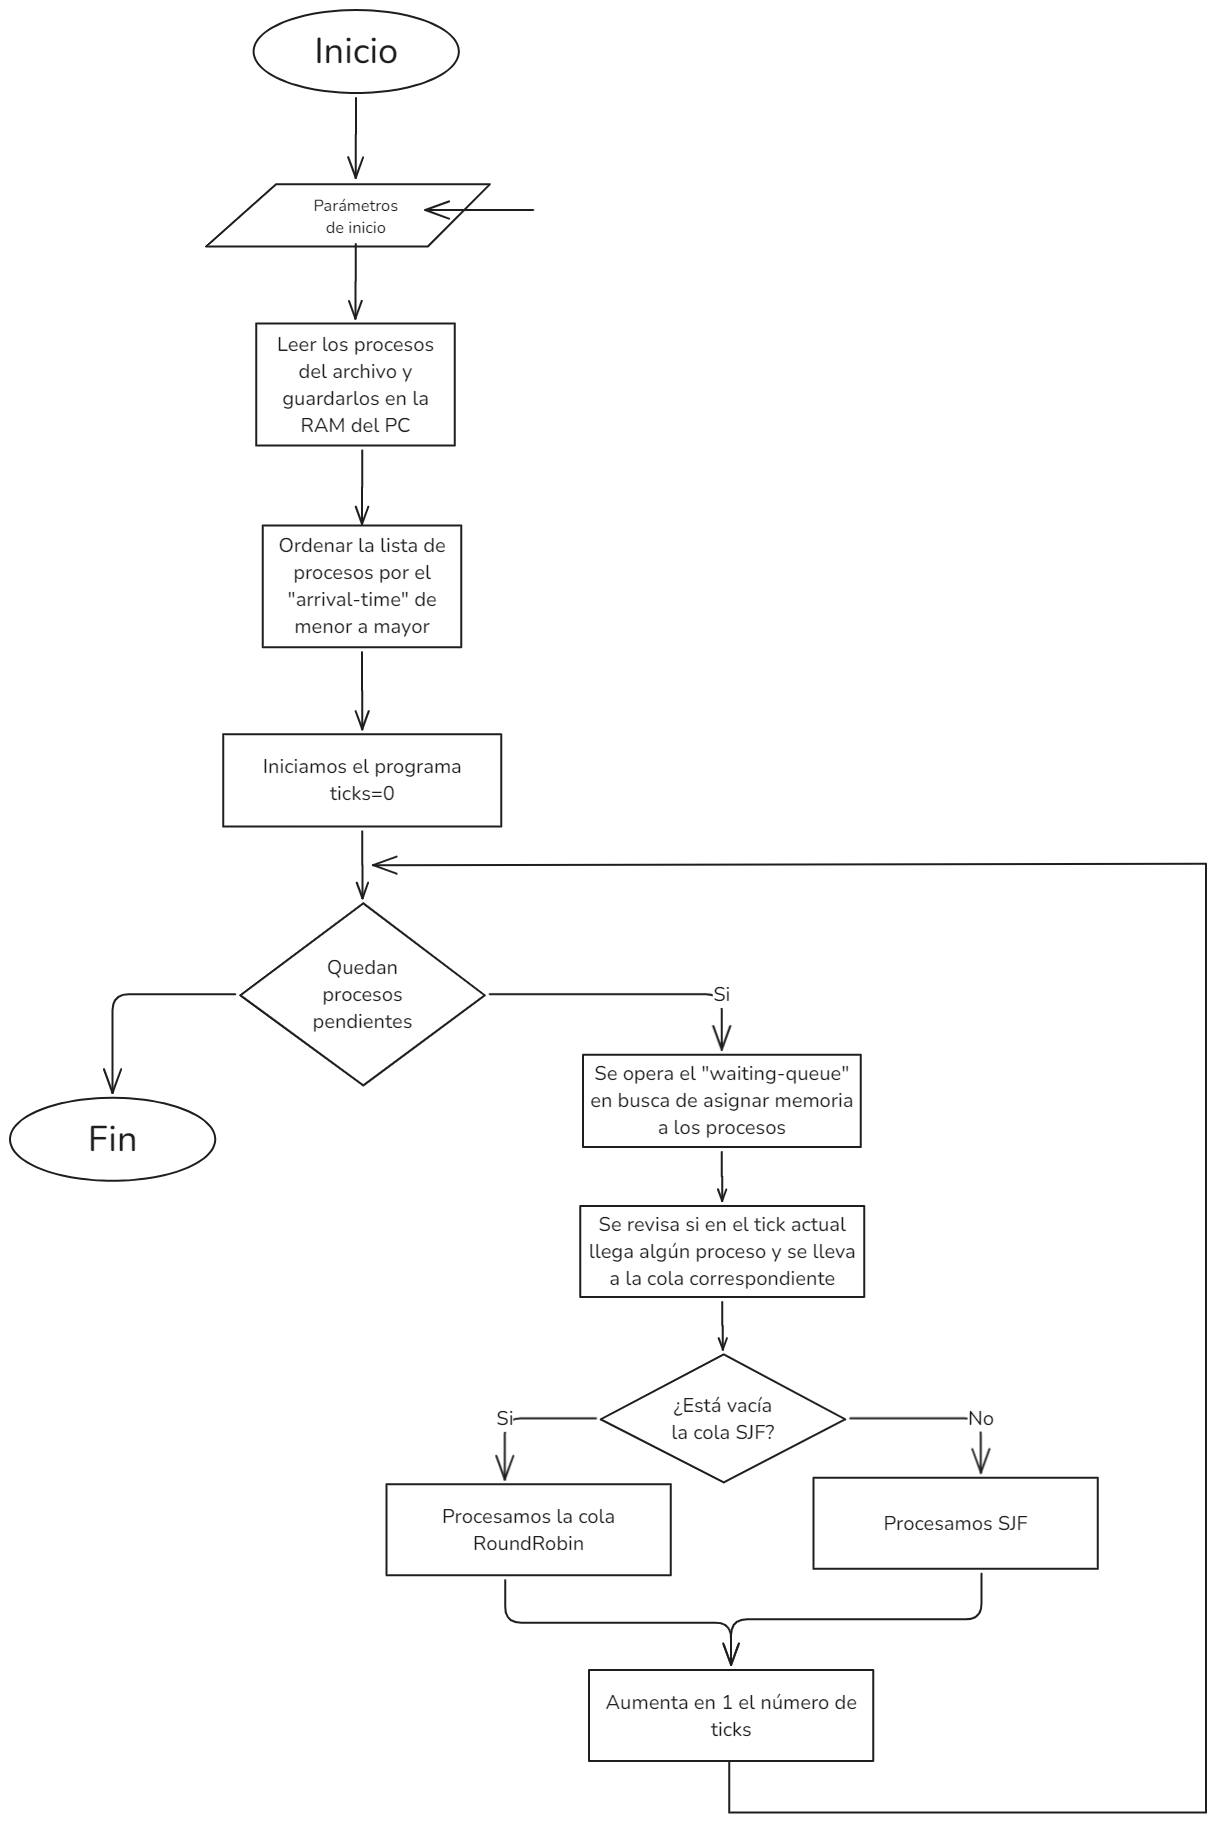
\includegraphics[height=12cm]{src/figures/Diagrama de flujo.png}
    \caption{Diagrama de flujo del desarrollo de forKing}\label{fig:flowchart}
\end{figure}


    \newpage
    \section{Implementación}
La implementación de los diversos algoritmos y estructuras de datos fue realizada en el lenguaje de programación C. Las diferentes funciones y estructuras fueron implementadas en archivos separados, con el objetivo de mantener una estructura de directorios clara y ordenada. A continuación se detallara esta implementación.

\subsection{Estructura de directorios}
Dentro del directorio \texttt{src} se encuentran los siguientes archivos:
\begin{itemize}
    \item \texttt{BuddySystem.c}: Contiene la implementación del algoritmo de asignación de memoria Buddy System.
    \item \texttt{errors.c}: Contiene la implementación de funciones para manejar errores.
    \item \texttt{files.c}: Contiene la implementación de funciones para manejar archivos.
    \item \texttt{forking.c}: Contiene las funciones para manejar \texttt{main} dentro del programa, utilizando las demás funciones y estructuras del proyecto.
    \item \texttt{main.c}: Contiene la función \texttt{main} del programa.
    \item \texttt{process.c}: Contiene la implementación de funciones y estructuras de datos para manejar procesos.
    \item \texttt{queue.c}: Contiene la implementación de funciones y estructuras de datos para manejar colas.
    \item \texttt{utilities.c}: Contiene la implementación de funciones varias, de utilidad.
\end{itemize}

Dentro del directorio \texttt{testing}, se encuentran los archivos:
\begin{itemize} 
    \item \texttt{generator.c}: Contiene la función encargada del generador de ``procesos''.
    \item\texttt{gant\_creator.py}: Es un script de \textbf{Python} encargado de generar una carta gantt.
\end{itemize}
Por ultimo, dentro del directorio \texttt{incs} se encuentran las cabeceras incluidas en todos los archivos \texttt{.c}.


\subsection{Estructuras de datos}
Las estructuras de datos utilizadas fueron las siguientes:
\subsubsection*{Lista enlazada simple}
Esta se encuentra implementada con la estructura \texttt{ProcessNode}, el cual contiene las variables:
\begin{itemize}
    \item \texttt{Process data}: Donde se almacenarán los procesos
    \item \texttt{Position next}: Puntero al nodo siguiente de la lista
\end{itemize}
La lista enlazada simple se utilizo para almacenar y ordenar los procesos ingresados en el programa según su \textit{arrival time}, el ordenamiento de la lista se realizo en primer instancia con \textit{bubble sort}, sin embargo al probar el programa en cantidades grandes, lo ineficiente de este algoritmo salio a flote, debido a que se encontró con tiempos de espera extensos al ejecutar el programa. A raíz de de esto se decidió implementar el algoritmo \textit{merge sort}, el cual redujo sustancialmente la cantidad de tiempo de demora del programa en ordenar los datos.

Esta estructura de datos es la encargada de almacenar los procesos en memoria, con esto las demás estructuras unicamente deben utilizar punteros a estos datos, ahorrando una cantidad significativa de espacio.

\subsubsection*{Colas}
Las colas se encuentran implementadas con la estructura \texttt{CircularNode}, la cual, en realidad es una \textit{lista circular doblemente enlazada} en donde el \textit{rear} y el \textit{front} de la cola son representadas por el nodo anterior y siguiente del centinela de la lista. Este contiene las variables:
\begin{itemize}
    \item \texttt{Process* process}: Puntero al proceso almacenado. Este puntero apunta a algún proceso contenido en la lista enlazada simple anterior
    \item \texttt{PtrToCircularNode next}: Puntero al nodo siguiente de la lista
    \item \texttt{PtrToCircularNode prev}: Puntero al nodo anterior de la lista
\end{itemize}

La implementación de las colas fue fundamental para el funcionamiento del programa, ya que sus características permiten manejar fácilmente el flujo y orden de los procesos. Las colas fueron usadas en el:
\begin{itemize}
    \item Arrival Queue
    \item Waiting Queue
    \item SJF
    \item RoundRobin
\end{itemize}


Para insertar elementos en las colas existe la función estándar de \texttt{enqueue}, la cual simplemente ingresa un elemento en la cola, sin embargo por motivos de comodidad y para cumplir con el funcionamiento deseado se incluyo la función \texttt{sorted\_enqueue}, la cual se encargo de ingresar decreciente o crecientemente  un proceso en cola según un criterio dado. Por ejemplo al ingresar en  SJF se ingresa según su \textit{burstime}.

\subsubsection*{Arboles binarios}
Los arboles binarios se encuentran implementados en la estructura \texttt{\_treeNode} , definida por las siguientes variables:
\begin{itemize}
    \item \texttt{Buddy element}: Corresponde  a una estructura la cual contiene un puntero a proceso, la altura del elemento dentro del arbol y una banera que indica el estado de uso del elemento, representadas por: \texttt{Process* process}, \texttt{unsigned int order} y \texttt{isUsed} respectivamente.
    \item \texttt{TreePosition parent}: Puntero a nodo el cual representa al nodo padre.
    \item \texttt{TreePosition left}: Puntero a nodo que representa al hijo izquierdo.
    \item \texttt{Treeposition right}: Puntero a nodo que representa al hijo derecho.
\end{itemize}

El árbol binario fue implementado en el \textit{BuddySystem},  asignando ``memoria'' inteligentemente mediante el operaciones relacionadas a las potencias de dos y logaritmos en base dos, con el fin de decidir el espacio optimo del proceso entregado según su memoria requerida. Inicialmente estas operaciones se realizaron matemáticamente, mediante funciones de la biblioteca \texttt{math.h} sin embargo se opto por realizarlas de forma binaria, lo que disminuyo la carga del programa, haciéndolo mas eficiente.


\subsection{Algoritmos de planificacion}
Como ya fue mencionado anteriormente los algoritmos de planificación utilizados fueron \texttt{Shortest Job First y Round Robin}. Su implementación consistió en:

\begin{itemize}
    \item \textbf{Shortest Job First}: Para la implementación del algoritmo \textit{SJF} se utilizo una cola a través de una lista circular doblemente enlazada, esta cola se ordeno mediante la función \texttt{sorted\_enqueue}, realizando comparaciones con el \textit{burstime} del proceso que esta siendo trabajado (en caso de que la cola que este siendo procesada sea \textit{SJF}) con el proceso ingresado.

    \item \textbf{Round Robin}: En el caso de la cola \textit{Round Robin}, esta se trabajó con la misma estructura de datos que el \textit{SJF}, sin embargo el funcionamiento de esta consiste en revisar el \textit{burstime} del proceso a ser trabajado, se realiza una comparación para ver si es igual o mayor que el \textit{Quantum}, de ser asi se asigna a esta cola y este proceso es trabajado la cantidad de ticks que indica el \textit{Quantum}. Al llegar al final del \textit{Quantum} se verifica si el proceso debe pasar o no a la cola \textit{SJF} mediante una comparación simple.
\end{itemize}

\subsection{Otros ejecutables}

Otros programas utilizados en la ejecución del programa fueron un generador de procesos y parámetros y un generador de carta gant. El primer programa corresponde a un generador simple de procesos, el cual entrega parámetros aleatorios entre ciertos valores dados por el usuario mediante terminal.

\lstinputlisting[caption=Ejemplo de entrada forKing, label={lst:exampleInput}]{src/input.txt}


Mientras que el generador de carta Gantt utiliza el lenguaje de programación \textbf{Python} con las librerias \texttt{matplotlib, numpy y random}, leyendo un archivo tipo csv el cual se genera al ejecutar el programa principal.

\begin{figure}[!ht]
    \centering
    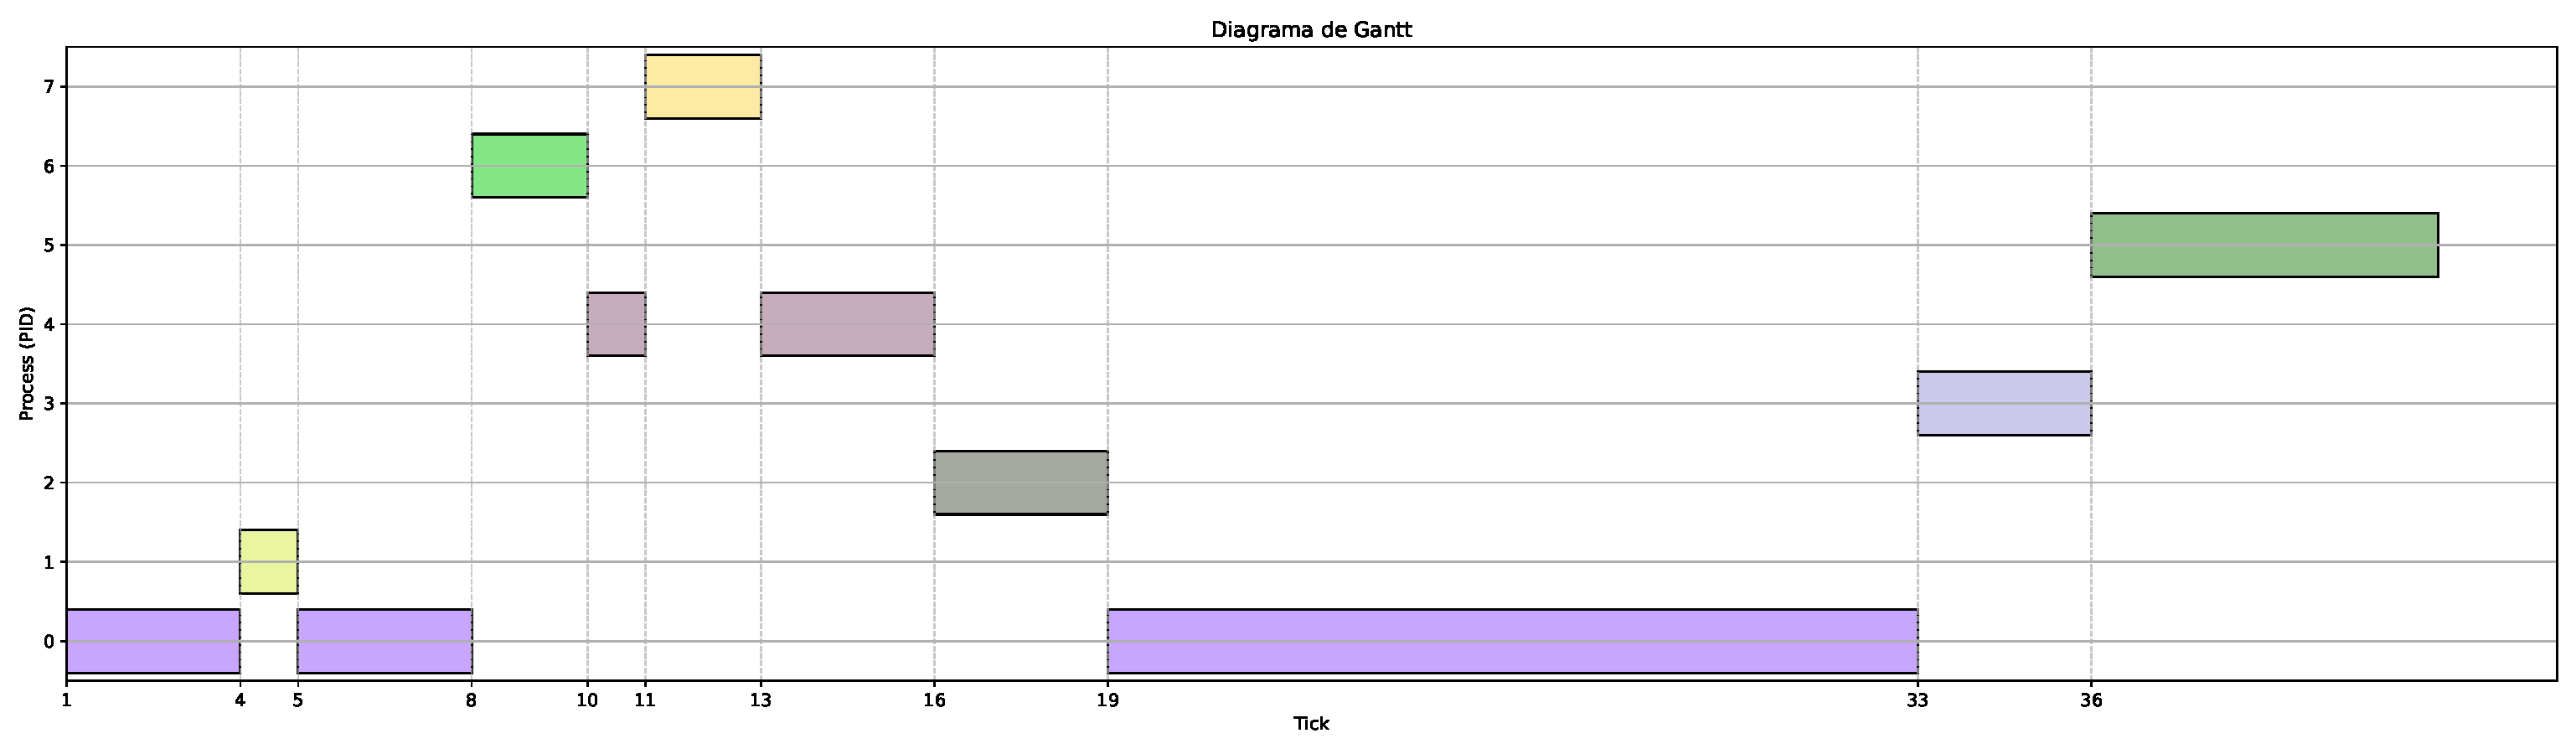
\includegraphics[width=\textwidth]{src/figures/carta_gant.pdf}
    \caption{Ejemplo de carta Gantt con forKing}\label{fig:gantt}
\end{figure}
    \newpage
    \section{Gestión del equipo de trabajo}
\rhostart{E}l equipo de trabajo constó de 3 personas, entre las cuales se tomaron las decisiones y se distribuyeron las tareas. Para un mejor orden y eficiencia, se establecieron normas de codificación, se acordó trabajar mediante una lista de tareas pendientes y realizar reuniones semanales.

\subsection{Normas de codificación}
En lo que respecta el nombramiento de variables, las constantes fueron llamadas con el formato \verb|SCREAMING_SNAKE_CASE|, y las variables con \verb|camelCase|.


\begin{lstlisting}[language=C, caption=Ejemplo de Screaming Snake Case y camelCase]
#define CLEAR_SCREEN "\033[H\033[J"
unsigned int arrivalTime;
\end{lstlisting}

Se acordó nombrar a las funciones con el formato \verb|snake_case|, y colocar sus llaves de apertura debajo de su prototipo.

\begin{lstlisting}[language=C, caption=Ejemplo de Snake case]
void delete_list(List L)
{
    Position P, Tmp;
    P = L->next;
    L->next = NULL;
    while(P!= NULL){
        Tmp = P->next;
        free(P);
        P = Tmp;
    }
}
\end{lstlisting}

Por otro lado las llaves de apertira de otros bloques de código se colocaron justo al lado de su línea final, evitando omitir las llaves cuando existiese una única sentencia.

\begin{lstlisting}[language=C, caption=Ejemplo bloques de código]
if(!clean){
    // Imprimir Informacion final
    print_program(&forkingConfig, forkingStatus);
}
\end{lstlisting}

Por último, para los archivos de cabecera se acordó usar guardias, con el nombre de su archivo en \verb|SCREAMING_SNAKE_CASE|.

\begin{lstlisting}[language=C, caption=Ejemplo de Guardias en archivos de cabecera]
#ifndef PROCESS_H
#define PROCESS_H
\end{lstlisting}

\subsection{Lista de tareas y organización}
Una vez establecida una norma de codificación común, se establecieron objetivos a corto, mediano y largo plazo, los cuales fueron listados para mantener un control del flujo de trabajo y repartirlos; por ejemplo, el primer objetivo fue crear las estructuras de datos necesarias (colas, listas enlazadas y árbol binario), por lo que se le encargó a cada integrante la codificación de una de ellas.

\subsection{Reuniones semanales}

Se fijaron semanalmente días y horarios de trabajo en conjunto, con el objetivo de discutir y/o fijar los objetivos del proyecto, resolver problemas de código mayores, o simplemente avanzar con Las tareas fijadas cada uno por separado; estas reuniones se hicieron de forma tanto presencial como asincrónicas a través de videollamadas y la herramienta LiveShare\footnote{Extensión de Visual Studio Code que permite el trabajo paralelo en un entorno virtual.} para codificar en conjunto. Esta modalidad fue extremadamente útil, pues se mantuvo una buena consistencia y flujo de avances semanales, en poco tiempo cumpliendo en poco tiempo con buena parte de los objetivos autoimpuestos. Por otro lado, para tareas menores se permitió que cada uno trabajara individualmente en la tarea que estimase conveniente fuera de estos horarios establecidos.
    \newpage
    \section{Posibles Mejoras a futuro}
\rhostart{A} pesar de su correcta funcionalidad \textit{forKing} tiene algunas limitaciones que podrían ser mejoradas en el futuro así como caracteristicas que podrían mejorar su funcionalidad pero que, por distintas razones, fueron omitidas; estas son las siguientes:
\begin{enumerate}
    \item \textbf{Ordenamiento de colas}: La cola \texttt{sjfQueue}, para su correcto funcionamiento debe estar ordenada de tal manera que el proceso que se encuentra al inicio de la misma sea aquel de la cola con el menor \texttt{burstTime}; este es también el caso de la cola \texttt{WaitingQueue} donde el primer proceso debe ser el de menor requerimiento de memoria.
    El proceso usado para conseguir este resultado tiene una complejidad de $O(n)$, sin embargo no se encontró una manera más eficiente de conseguirlo.
    Lo anterior ocasiona que para cantidades de procesos muy grandes la simulación pueda tardar mucho tiempo en ejecutarse.
    \item \textbf{Uso ineficiente del BuddySystem}: El \textit{BuddySystem} a pesar de solucionar la mayoría de problemas de asignación de memoria tiene un defecto clave: Depende de espacios con potencias de dos, esto ocasiona que si un proceso requiere $1025$ bytes de memoria, el \textit{BuddySystem} tendrá que asignar $2048$ bytes de memoria a dicho proceso, desperdiciando $1023$ bytes de memoria.
    Esto podría solucionarse complejizando más el algoritmo de asignación de memoria.
    \item \textbf{Trabajo con hebras y/o procesos paralelos}: Una de las ideas más ambiciosas surgida en los inicios del desarrollo de forKing fue el trabajar con procesos paralelos, mediante el uso de \textit{hebras}\footnote{Unidad más pequeña de ejecución dentro de un proceso, que permite realizar tareas concurrentes compartiendo la memoria del proceso principal} o, de procesos generados con \texttt{fork()}\footnote{Funcion estandar de la libreria ``unistd.h'', la cual permite generar procesos hijos. \parencite{fork_function}} (de ahí el nombre del proyecto), sin embargo dada la complejidad de esta implementación y el tiempo con el que se contaba para la realización del proyecto se prefirió no enforcar los esfuerzos en dicha dirección.
    \item \textbf{Bloqueo de procesos, espera y ráfagas de E/S}: Durante el inicio de este proyecto se realizó una simplificación de lo que un simulador de un gestor de memoria y planificación de procesos debería hacer, en esta etapa se simplificó su funcionamiento dejando de lado algunas características como:
    \begin{itemize}
        \item \textbf{Bloqueo de procesos}: Se decidió no tener en cuenta el bloqueo de procesos, donde un proceso podría necesitar de la previa ejecución de otro para proceder con su ejecución.
        \item \textbf{Ráfagas de E/S}: En sistemas operativos reales un proceso no necesita un único \textit   {burstTime} para su completa ejecución sino que puede requerir de varias ráfagas de CPU combinadas con ráfagas de E/S, por lo que se decidió no tener en cuenta esta característica.
    \end{itemize}
\end{enumerate}
















    \section{Conclusiones}

A raíz de la realización de este proyecto se pudo comprender de mejor manera los usos reales de las estructuras de datos analizadas durante las clases. Además fue posible evidenciar la importancia de los conceptos introducidos por estas estructuras para el desarrollo de nuevas estructuras como el caso del \textit{BuddySystem}.

Puesto que este proyecto permitió el trabajo con grandes volúmenes de datos se comprendió de mejor manera los conceptos de eficiencia de algoritmos como el \texttt{Merge Sort} en contra de los algoritmos de ordenamiento de listas como \texttt{Bubble Sort}. Así como la importancia de la creación de funciones eficientes para el manejo de las diferentes estructuras de datos.

Además, al tratarse de una simulación de un gestor de procesos y de memoria se pudo comprender mejor el funcionamiento de algoritmos como \texttt{Round Robin} y \texttt{Shortest Job First}, los cuales son usados en muchos de los sistemas operativos modernos.

    \newpage
    \nocite{*}
    \printbibliography
\end{document}













% \section{Title}

%     The \verb|\maketitle| command generates the title information, abstract and corresponding author information. The following sections describe each of these.

%     In addition to the \verb|\title| command, a new command named \verb|\journalname| has been added to include more information. 

%     If you do not need this command, you can undefined it and the content will be adjusted automatically.

%     \subsection{Abstract}

%         The abstract is placed with \verb|\begin{abstract} \end{abstract}| command and is declared in the preamble. Then, the keywords are placed with the command \verb|\keywords{}|. If the keywords are not declared in the preamble, the content will be adjusted automatically.

%     \subsection{Corresponding author}

%         Rho includes a section for corresponding author information. In this section you can easily add important information about your article, such as doi, publication dates, and license.

%         If you do not need this section, you can disable it directly from the main.tex. Set \textit{false} in \verb|\setbool{corres-info}{true/false}|. The content will be adjusted automatically and no modifications to the class document will be necessary.
        
%         If you want this section but, for example, you do not need the doi, just do not declare the command in the preamble and the content will be adjusted automatically.

% \section{Other elements}

%     \subsection{Lettrine}
    
%         The \verb*|\rhostart{}| command provides a personalized lettrine for the beginning of a paragraph as shown in this document example.

%     \subsection{Line numbering}

%         By implementing the \textit{lineno} package, the line numbering of the document can be placed with the command \verb|\linenumbers|. 
		
%         I recommend placing the command after the table of contents for a better appearance (comment or delete if not required).

% \section{Equation}

%     Equation \ref{ec:equation}, shows the Schrödinger equation as an example. 
%         \begin{equation} \label{ec:equation}
%             \frac{\hbar^2}{2m}\nabla^2\Psi + V(\mathbf{r})\Psi = -i\hbar \frac{\partial\Psi}{\partial t}
%         \end{equation} 
%     The \textit{amssymb} package was not necessary to include, because stix2 font incorporates mathematical symbols for writing quality equations. In case you choose another font, uncomment the package in \textit{rho class}.

%     In case you want to change the values that adjust the spacing above and below in the equations, go to \textit{rho-class/rho.cls/math packages} section and play with \verb|\setlength{\eqskip}{8pt}| value until the preferred spacing is set.

% \section{Rho packages}

%     \subsection{Rhoenvs}
    
%         This template has its own environment package \textit{rhoenvs.sty} designed to enhance the presentation of information within documents. Among these custom environments are \textit{rhoenv}, \textit{info} and \textit{note}.
    
%         There are two environments which have a predefined title. These can be included by the command \verb|\begin{note}| and \verb|\begin{info}|. All the environments have the same style.
    	
%         An example using the rho environment is shown below.
    
%         \begin{rhoenv}[frametitle=Environment with custom title]
%             Hello! I am an example of the \textit{rhoenv} included in rhoenvs \LaTeX\ package. Here you can include relevant information or notes about your work. You can modify my title directly in the code.
%         \end{rhoenv}
    
%         Rhoenv is the only environment that you can customize its title. On the other hand, \textit{info} and \textit{note} adapt their title to Spanish automatically when the language package is defined.

%     \subsection{Rhobabel}

%         In this new version, we have included a package called \textit{rhobabel}, which have all the commands that automatically translate from English to Spanish when this language package is defined. 
        
%         By default, rho displays its content in English. However, at the beginning of the document you will find a recommendation when writing in Spanish. 
		
%         \textit{Note:} You may modify this package if you want to use other language than English or Spanish. This will make easier to translate the document without having to modify the class document.

% \section{Figures and tables}

%     \subsection{Sample figure}

%         Figure \ref{fig:figure} shows an example figure.
        
%             \begin{figure}[H]
%                 \centering
%                 \includegraphics[width=0.71\columnwidth]{src/figures/Example.pdf}
%                 \caption{Example figure obtained from PGFPlots \cite{PFGPlots}.}
%                 \label{fig:figure}
%             \end{figure}

%     \subsection{Sample double figure}

%         Figure \ref{fig:examplefloat} shows an example of a two-picture floating figure that covers the width of the page. It can be positioned at the top or bottom of the page. The space between the figures can also be changed using the \verb|\hspace{Xpt}| command.

%         \begin{figure*}[!t] % t for position at the top of the current page; b for position at the bottom of the current page
%             \centering
%                 \begin{subfigure}[b]{0.38\linewidth} % Fig (a)
%                     \includegraphics[width=\linewidth]{src/figures/example2.pdf}
%                     \caption{Example left figure.}
%                     \label{fig:figa}
%                 \end{subfigure}
%             \hspace{15pt}   % Space between the figures
%                 \begin{subfigure}[b]{0.38\linewidth} % Fig (b)
%                     \centering
%                     \includegraphics[width=\linewidth]{src/figures/example2.pdf}
%                     \caption{Example right figure.}
%                     \label{fig:figb}
%                 \end{subfigure}
%             \caption{Example figure that covers the width of the page obtained from PGFPlots \cite{PFGPlots}.}
%             \label{fig:examplefloat}
%         \end{figure*}

%     \subsection{Sample table}

%         In the same way as the figures, you can place tables in one or two columns, depending on the length of the table.

%         Table \ref{tab:table}, shows an example table that covers the width of the page positioned at the bottom of a new page.

%         \begin{table*}[h]
%             \RaggedRight
%             \caption{Table example that covers the width of the page.}
%             \label{tab:table}
%                 \begin{tabular}{lllp{12.2cm}}
%                     \toprule
%                     \textbf{Day} & \textbf{Min Temp} & \textbf{Max Temp} & \textbf{Summary} \\ 
%                     \midrule
%                     Monday & 11\textdegree C & 22\textdegree C & A clear day with lots of sunshine.  Strong breeze will bring down the temperatures. \\
%                     Tuesday & 9\textdegree C & 19\textdegree C & Cloudy with rain, across many northern regions. \\
%                     Wednesday & 10\textdegree C & 21\textdegree C & Rain will still linger for the morning. 
%                     Conditions will improve by early afternoon and continue 
%                     throughout the evening.\\
%                     \bottomrule
%                 \end{tabular}

%             \tabletext{Note: Obtained from \LaTeX\ tables \cite{projects-2023}.}

%         \end{table*}

%         %\newpage
% \section{Codes}

%     This class\footnote{Hello there! I am a footnote :)} includes the \textit{listings} package, which offers customized features for adding codes specially for C, C++, \LaTeX\ and Matlab. You can customize the format in \textit{rho class} file.

%     \nolinenumbers
%     \lstinputlisting[caption=Example of matlab code., label={lst:listing-Mat}, language=Matlab]{src/example.m}
%     \linenumbers

%     If line numbering is enabled, we recommend placing the command \verb|\nolinenumbers| at the beginning and \verb|\linenumbers| at the end of the code. 

%     This will temporarily remove line numbering and the code will look better.

% \section*{Unnumbered section} \label{sec:unsec}

%     If a unnumbered section is declared, a square appears followed by the section name. This style is characteristic of this class and is only for first level sections.

%     Since this affects the title of the table of contents and references, you can make a modification in \textit{rho-class/rho.cls/section style} to remove the square. See appendix for more information.

% \section{Table of contents}

%     The ToC provides a preview of the content and its location in the document. Uncomment the command \verb|\tableofcontents| to display it. Remember that unnumbered sections will not appear in the ToC, however, you can place them manually with the command \verb|\addcontentsline{toc}{section}{section name}|.

%     See the appendix section for more information. There, you will find recommended modifications to adjust the table of contents when unnumbered sections are defined.

% \section{Reference style}

%     The default formatting for references follows the IEEE style. At the end of the document, you will find an example of the default reference formatting.

%     You can modify the style of your references, for that, go to \textit{rho-class/rho.cls/biblatex}. See appendix for more information.

% \section{Appendix}

%     \subsection{Unnumbered sections}

%         As mentioned in section \ref{sec:unsec}, when placing a first level section without number a square appears followed by the section name. In case you do not require this extra detail, you can make the following modification.

% \nolinenumbers
% \begin{lstlisting}[language=TeX, caption=Alternative unnumbered section.]
% \titleformat{name=\section,numberless}[block]
%     {\color{rhocolor}\sffamily\large\bfseries}
%     {}
%     {0em}
%     {#1}
%     []
% \end{lstlisting}
% \linenumbers

%         You can change to this code in \textit{rho-class/rho.cls/section style}. Once the document is recompiled, this square will disappear. 

%         Remember that this code affects the ToC and references title. To show rho class functionalities, this option is enabled by default.

%     \subsection{Table of contents}
    
%         In case you have chosen the unnumbered sections and you want to add the ToC, you can do the following to adjust the content.

% \nolinenumbers
% \begin{lstlisting}[language=TeX, caption=ToC when unnumbered section is chosen.]
% \setlength\tocsep{0pc}

% \titlecontents{section}[\tocsep]
%     {\addvspace{4pt}\sffamily\selectfont\bfseries}
%     {\contentslabel[\thecontentslabel]{\tocsep}}
%     {}
%     {\hfill\thecontentspage}
%     []

% \titlecontents{subsection}[1pc]
%     {\addvspace{4pt}\small\sffamily\selectfont}
%     {\contentslabel[\thecontentslabel]{\tocsep}}
%     {}
%     {\ \titlerule*[.5pc]{.}\ \thecontentspage}
%     []

% \titlecontents*{subsubsection}[1pc]
%     {\footnotesize\sffamily\selectfont}
%     {}
%     {}
%     {}
%     [\ \textbullet\ ]
% \end{lstlisting}
% \linenumbers

%         As you can see, the value of \verb|\tocsep| was changed to 0pc for the sections. For subsections and subsubsections the value was changed to 1pc.

%         By making this small modification, the contents of the ToC will look more organized.

%         If you use numbered sections, you do not need to make this modifications, unless you prefer other values.

%     \subsection{References and paths}

%         In case you require another reference style, you can go to \textit{rho-class/rho.cls/biblatex} and modify the following. 

% \nolinenumbers
% \begin{lstlisting}[language=TeX, caption=Reference code.]
% \usepackage[
%     backend=biber,
%     style=ieee,
%     sorting=ynt
% ]{biblatex}
% \end{lstlisting}

% %\linenumbers

%         By default, rho class has its own .bib for this example, if you want to name your own bib file, change the following path.

% \nolinenumbers
% \begin{lstlisting}[language=TeX]
% \addbibresource{rho.bib}
% \end{lstlisting}

% \begin{lstlisting}[language=C, caption=Here is an implementation of a delete function for a singly linked list in C.(\href{https://users.cs.fiu.edu/~weiss/\#dsaac2e}{Source code})]
%     /* Delete from a list */
% /* Cell pointed to by P->Next is wiped out */
%     /* Assume that the position is legal */
%     /* Assume use of a header node */

%     void
%     Delete( ElementType X, List L )
%     {
%         Position P, TmpCell;

%         P = FindPrevious( X, L );

%         if( !IsLast( P, L ) )  /* Assumption of header use */
%         {                      /* X is found; delete it */
%             TmpCell = P->Next;
%             P->Next = TmpCell->Next;  /* Bypass deleted cell */
%             free( TmpCell );
%         }
%     }
% \end{lstlisting}

% %\linenumbers

%     \subsection{Info environment}

%         We will show an example of the info environment declared in the ‘rhoenvs.sty’ package. Remember that \textit{info} and \textit{note} are the only packages that translate their title (English or Spanish).

%         \begin{info}
%             Small example of info environment.
%         \end{info}

% \section{Supporting}

%     Did you like this class document? Check out \href{https://www.overleaf.com/latex/templates/tau-class-lab-report-template/chhshmhxstsq}{tau class} designed for your lab reports.

%     \subsection*{Any contributions are welcome!}
    
%         Coffee keeps us awake and helps us create better \LaTeX\ templates. If you wish to support our work, you can do so through PayPal:\\
%         \url{https://www.paypal.me/GuillermoJimeenez}.
        
%         \begin{center}
%             Enjoy writing with rho \LaTeX\ class\hspace{5pt}\faChessKnight 
%         \end{center}

% \section{Contact us}

%     You can contact us through these methods.\\
    
%     \noindent\faWix\hspace{5pt}\href{https://memonotess1.wixsite.com/memonotess}{https://memonotess1.wixsite.com/memonotess} \\
%     \faEnvelope[regular]\hspace{7pt}memo.notess1@gmail.com \\
%     \faEnvelope[regular]\hspace{7pt}eduardo.gracidas29@gmail.com \\
%     \faGithub[regular]\hspace{7pt}srrathi
%     %\faInstagram\hspace{8pt}memo.notess

% %----------------------------------------------------------

% \printbibliography

% %----------------------------------------------------------
